%!TEX root = ../main.tex
\documentclass[../main.tex]{subfiles}

\begin{document}

  \chapter{Size Spectrum Theory}\label{chapter:sizetheory}

  In this chapter we consider the models in \cite{mckendrick1926} and \cite{foerster1959} who describe a system indexed by age. We consider the advances in \cite{silvert1978} who describe new equations indexed by weight and derive the standard McKendrick-von Foerster Equation for weight indexed systems.

  This work serves as the basis for \cite{datta2010}, who construct a stochastic model for the dynamics of population which they call the ``Deterministic Jump-Growth Equation''. We consider the similarities between this equation and the McKendrick-von Foerster Equation.

  \section{Age Indexed Models}
  \cite{mckendrick1926} first posed the idea of modelling biological processes for medicinal science by a single characteristic. In a process if individuals meet, they transfer information within the system and if we consider these individuals as particles in a system moving according to a dimension indexed by this single characteristic then their movement becomes a study in kinetics.

  \cite{foerster1959} extended the principle equations derived in \cite{mckendrick1926}. \cite{trucco1965} gives a rigorous discussion of the advancements made in \cite{foerster1959} and further considers the steady state solutions of what he calls ``The Von Foerster Equation''.

  \subsection{The Von Foerster Equation}
  The Von Foerster Equation was a major extension to the work of \cite{mckendrick1926}. It defines the standard in age indexed population models and reads

  \begin{equation}\label{theory:eq:vf}
    \frac{\partial n}{\partial t} + \frac{\partial n}{\partial a} = - m(a)n,
  \end{equation}

  for a mortality function dependent on age $m(a)$. We derive \autoref{theory:eq:vf} following the method discussed in \cite{trucco1965} based upon the discussion in \cite{foerster1959}. Suppose that $n(t, a)$ represents the density of individuals at time $t$ in the age category $[a, a + \Delta a)$, then

  \begin{eqnarray}\label{theory:eq:wordsvf}
    \frac{\partial}{\partial t} \left( n(a, t) \Delta a \right)
    &=& + \mbox{ rate of entry of } a \nonumber \\
    && - \mbox{ rate of departure at } (a + \Delta a) \nonumber \\
    && - \mbox{ deaths in } [a, a + \Delta a).
  \end{eqnarray}

  We can express \autoref{theory:eq:wordsvf} in mathematical terms for some \emph{flux}, $J(t, a)$, which describes the rate of movement of individuals in $[a, a + \Delta a)$ as

  \begin{equation}\label{theory:eq:flux}
    \frac{\partial n}{\partial t} = \frac{J(t, a) - J(t, a + \Delta a)}{\Delta a} - M \cdot n(a, t),
  \end{equation}

  for some per capita mortality rate $M([a, a + \Delta a))$. We take the \emph{flux}, $J$, to define the movements of individuals within the system. As individuals become older the flux can be assumed to be proportional to the density of individuals with some velocity $v(t, a)$. If the ageing corresponds to the passing of time then

  $$ v(t, a) = \frac{\partial a}{\partial t} = 1$$

  and so $J(t, a) = n(t, a)$. Substituting this into \autoref{theory:eq:flux} it is clear that in the limit as $\Delta a \to 0$, \autoref{theory:eq:flux} tends to \autoref{theory:eq:vf}.

  \section{The Transport Equation}\label{theory:sec:transport}
  After considering \autoref{theory:eq:vf} we consider a more general form of equation. Transport Equations, or convection-diffusion equations, take the general form

  \begin{equation}\label{theory:eq:transport}
    \frac{\partial u}{\partial t} = \nabla \cdot (D \nabla u) - \nabla \cdot (\vec{v} u) + R.
  \end{equation}

  They describe particles undergoing diffusion and convection. In one dimension \autoref{theory:eq:transport} reduces to

  \begin{equation}\label{theory:eq:transport1d}
    \frac{\partial u}{\partial t} = - \upsilon u_x + R + (D u_x)_x.
  \end{equation}

  Comparing the coefficient definitions from \cite{stocker2011} to the ideas from the derivation of \autoref{theory:eq:vf} we take $u$ as the quantity of interest (population or population density), then we can interpret each term in \autoref{theory:eq:transport1d}.

  The first term $-\upsilon u_x$ describes the convection (movement due to mass) in the system. $\upsilon$ describes the velocity particles in the system are moving at. This is analogous to the growth of individuals in the population, the rate at which they grow and move through the weight range.

  The second term $R$ describes the creation or destruction of $u$. In \autoref{theory:eq:vf} this becomes the death (naturally or predatorily) of the population.

  For the diffusion term $(D u_x)_x$, imagine that $c$ is the concentration of a chemical. When concentration is low somewhere compared to the surrounding areas (e.g. a local minimum of concentration), the substance will diffuse in from the surroundings, so the concentration will increase. The reverse case applies, also. This is analogous to phenomena that are exhibited in approximations the Jump-Growth Equation which we talk about in the next section.

  \section{Weight Indexed Models}
  \subsection{McKendrick-von Foerster Equation}\label{theory:sec:mvf}
  \cite{silvert1978} introduced a more general construction of the McKendrick-von Foerster Equation, notwithstanding a change from age indexed populations to sized based populations, in a model which allowed growth and mortality to be functions of body mass. Their changes are widely used in mathematical biology and a full derivation can be found in \cite{silvert1978}. However a simple argument is that the \emph{flux} described in \autoref{theory:eq:flux} is changed for a flux that depends on the growth of individuals

  \begin{equation}
    J(t, w) = g(t, w) n(t, w)
  \end{equation}

  and $m(a)$ becomes a mortality function in weight rather than age $\mu(w)$. Thus the McKendrick-von Foerster Equation reads

  \begin{equation}\label{theory:eq:mvf}
    \frac{\partial n}{\partial t} + \frac{\partial}{\partial w} \left(g \cdot n \right) = - \mu \cdot n.
  \end{equation}

  Considering this equation in the context of \autoref{theory:sec:transport} we can see \autoref{theory:eq:mvf} is a Transport Equation with no diffusion term. While a Transport Equation is defined on the region of $\mathbb{R^+} \times \mathbb{R}$, simply requiring an initial condition, the Von Foerster Equation is only defined on $\mathbb{R^+} \times \mathbb{R^+}$, thus requiring a left boundary condition along the line $(t, 0)$. Generally this boundary condition is defined as the births across the population which could simply be defined with

  \begin{equation}\label{theory:eq:simpleboundary}
    u(t, 0) = 0.
  \end{equation}

  This would be an uninteresting problem since the system would only include growth and death, but no birth. Thus instead of \autoref{theory:eq:simpleboundary} we introduce a birth rate $b(w)$ and integrate over the population to give a boundary condition

  \begin{equation}\label{theory:eq:boundary}
    u(t, 0) = \int_0^{\infty} b(w) u(t, w) \: \mathrm{d}t.
  \end{equation}

  Numerical methods cannot handle the domain $[0, \infty]$ and thus we need to introduce a right hand boundary condition at some weight $W$. This will be dealt with in due course.

  \subsection{Jump-Growth Equation}\label{theory:sec:jumpgrowth}
  While the mathematical framework presented in \cite{silvert1978}, \cite{datta2010} presents a different method of describing weight indexed population under the assumption that predation is a Markov process. The predation event extends the ideas of \cite{silvert1980} where predation is modelled by coupling the death of an individual in one weight interval $[w, w + \Delta w)$ with the growth of an individual in a different weight interval $[w', w' + \Delta w)$. This is illustrated in \autoref{theory:fig:predation} where we see there are three types of predation to yield `new' individuals.

  \begin{figure}[ht]
    \centering
    \caption{The death of an individual with weight $w_b$ is attributed to the growth of another individual with weight $w_a$ who dies to yield a new individual with weight $w_c = w_a + K w_b$ for some predation efficiency $K$. Taken from from \cite{datta2010}. \label{theory:fig:predation}}
    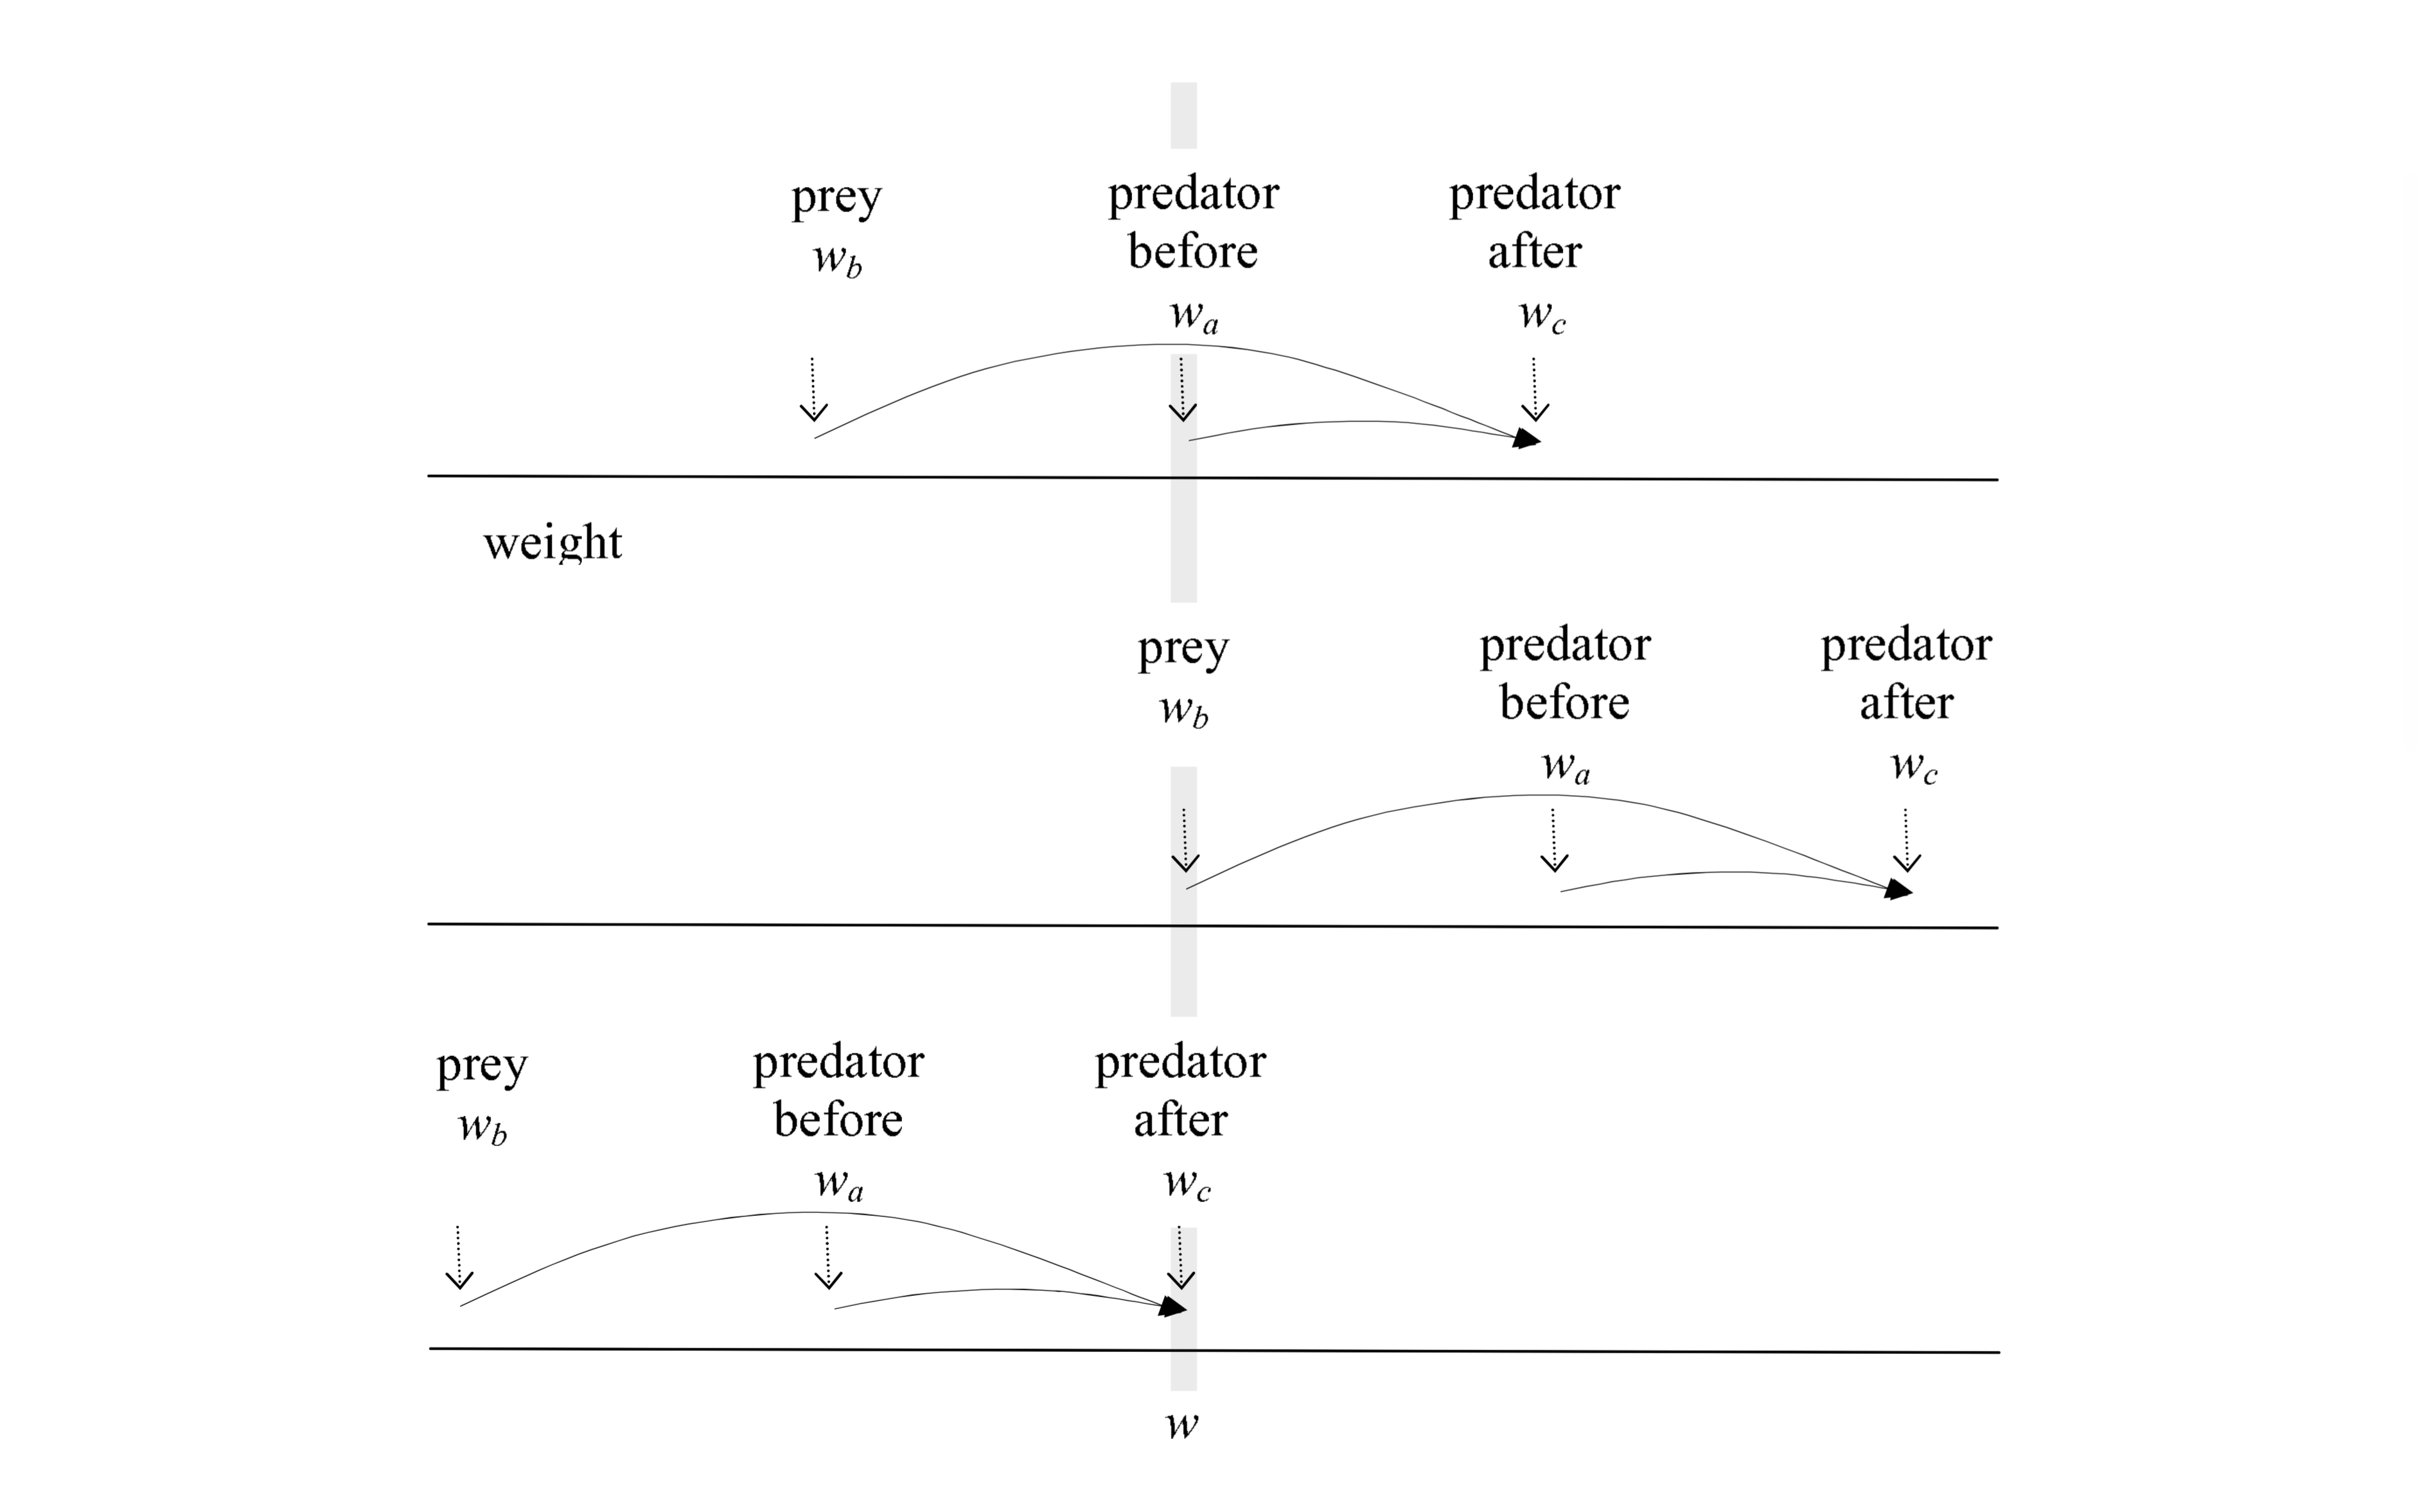
\includegraphics[width=0.75\textwidth]{_assets/stochastic_predation.png}
  \end{figure}

  Resolving the macroscopic behaviour of these predation events yields the deterministic equation

  \begin{equation}\label{theory:eq:discretejump}
    \frac{\partial \varphi_i}{\partial t} = \sum_j \left(- k_{ij} \varphi_i \varphi_j - k_{ji} \varphi_j \varphi_i + k_{mj} \varphi_m \varphi_j \right),
  \end{equation}

  where $m$ is the index satisfying the weight bracket $w_m \leq w_i - K w_j < w_{m+1}$ and $k_{xy}$ is the rate of predation events, indexed predator before prey. \cite{datta2010} explains that these three terms correspond to the three types of predation event seen in \autoref{theory:fig:predation}: losses from bracket $i$ (negative terms) occur because individuals in this bracket eat prey and become heavier and because these individuals are themselves eaten. Gains into weight bracket $i$ (the positive term) occur through smaller predators growing into this bracket by eating prey.

  We can create an analytic equation for use in calculations by taking the continuum limit of \autoref{theory:eq:discretejump} and using a continuous feeding rate function $k(w, w')$ to replace the rate constants $k_{xy}$. Thus \autoref{theory:eq:discretejump} becomes
  \begin{align}\label{theory:eq:jumpgrowth}
    \frac{\partial \phi(w)}{\partial t}
    = \int ( &- k(w', w) \phi(w)\phi(w') \nonumber \\
    & - k(w, w')\phi(w')\phi(w) \nonumber \\
    & + k(w - Kw', w')\phi(w - Kw')\phi(w')) \: \mathrm{d}w'.
  \end{align}

  \cite{datta2010} defines \autoref{theory:eq:jumpgrowth} as the ``Deterministic Jump-Growth Equation'' and again the three terms represent the methods of transferring weight within in the system through predation corresponding to the methods in \autoref{theory:fig:predation}: Predation on prey to become larger, being predated and being fed the correct weight to increase.

  \subsection{McKendrick-von Foerster Equation with Diffusion}\label{theory:sec:mvfdiffusion}
  The McKendrick-von Foerster Equation can be shown to be an approximation to the Jump-Growth Equation, but only to first order. A second order approximation can be yielded by including a diffusion term. If we consider the third term in the Jump-Growth Equation as a Taylor Series, then

  \begin{align}
    k(w - Kw', w')\phi(w - K w')
    = & k(w, w') \varphi(w) \nonumber \\
      & + (-K w') \frac{\partial}{\partial w} \left(k(w, w')\varphi(w')\varphi(w)\right) \nonumber \\
      & + \frac{1}{2}(-K w')^2 \frac{\partial^2}{\partial w^2} \left(k(w, w')\varphi(w)\right) + ...
  \end{align}

  Once this is substituted back into \autoref{theory:eq:jumpgrowth}
  \begin{align}\label{theory:eq:jumpdiffusion}
    \frac{\partial \phi(w)}{\partial t}
    & = \int - k(w', w) \phi(w)\phi(w')  \: \mathrm{d}w' \nonumber \\
    & - \frac{\partial}{\partial w} \int K w' k(w, w')\varphi(w)\varphi(w') \: \mathrm{d}w' \nonumber \\
    & + \frac{1}{2}\frac{\partial^2}{\partial w^2} \int (K w')^2 k(w, w')\varphi(w)\varphi(w') \: \mathrm{d}w' + ...
  \end{align}

  which can be seen as an approximation to the McKendrick-von Foerster Equation, with a diffusion term added. Thus for an appropriate choice of coefficients we can restrict our attention to equations in a Transport Equation form

  \begin{equation}\label{theory:eq:jumptransport}
    \frac{\partial u}{\partial t} = - (g \cdot u)_w - \mu \cdot u + \frac{1}{2}(D u)_{xx}.
  \end{equation}

  \section{Summary}
  In this chapter we have introduced the mathematical framework that will be used to model populations and shown that the macroscopic stochastic Jump-Growth equation is comparable to the Transport Equation form of the McKendrick-von Foerster Equation. In \autoref{chapter:modelequations} we introduce a numerical construction of the coefficients giving rise to the true models that will be solved in \autoref{chapter:method}.

\end{document}
